\FILE{section-usecases.tex}

\section{Use Cases for Analytics Services}
\label{sec:usecases}


\subsection{Use Case Development Process}

To specify use cases for our analytics framework, we encourage contributors to contact us and provide us with their high-level descriptions of their use cases. The use cases should be focusing on highlighting one or multiple aspects of the features related to analytics frameworks. While inspecting the various features we intend to collect and analyze them in various contexts that are relevant for analytics users. The lessons learned from this analysis are to be integrated into this document in order to formulate a comprehensive vendor neutral analytics framework.
Use cases can be formulated in various format but should include diagrams that make them easy to comprehend as well as allowing the reader to extract the specific analytical aspects. Such diagrams can include functional cross diagrams, process diagrams and others.
Use cases should especially address the use of metadata describing the functional and the data related properties. This includes metadata related to time, space, exchange/protocols, privacy, and security related aspects.
A functional description of the use case is to be included as a subsection called Functionalities and Activities. This section is mirroring our experience with documenting use cases as part of the Big Data Application Provider of NBDIF Reference Architecture. Hence, we assume the following draft form for a use case:

\begin{description}
\item[Title:] 		Title of the use case
\item[Contributor:] 	The list co contributors
\item[Description:] 	One to two sentences about major functionalities and activities with respect to the sample cross-functional diagram
	
	\begin{description}
	\item[Cross-Functional Diagram:]
		Inclusion of a cross functional Diagram, alternatively other diagrams could be 			chosen.
	\item[Functionality Activities:]
	\begin{enumerate}
        \item Activity \#1 -- description ...
        \item ...
        \item Activity \#n -- description ...
    	\item Use Case Summaries
    \end{enumerate}
\end{description}
\end{description}

\begin{figure}[htb]
    \centering
    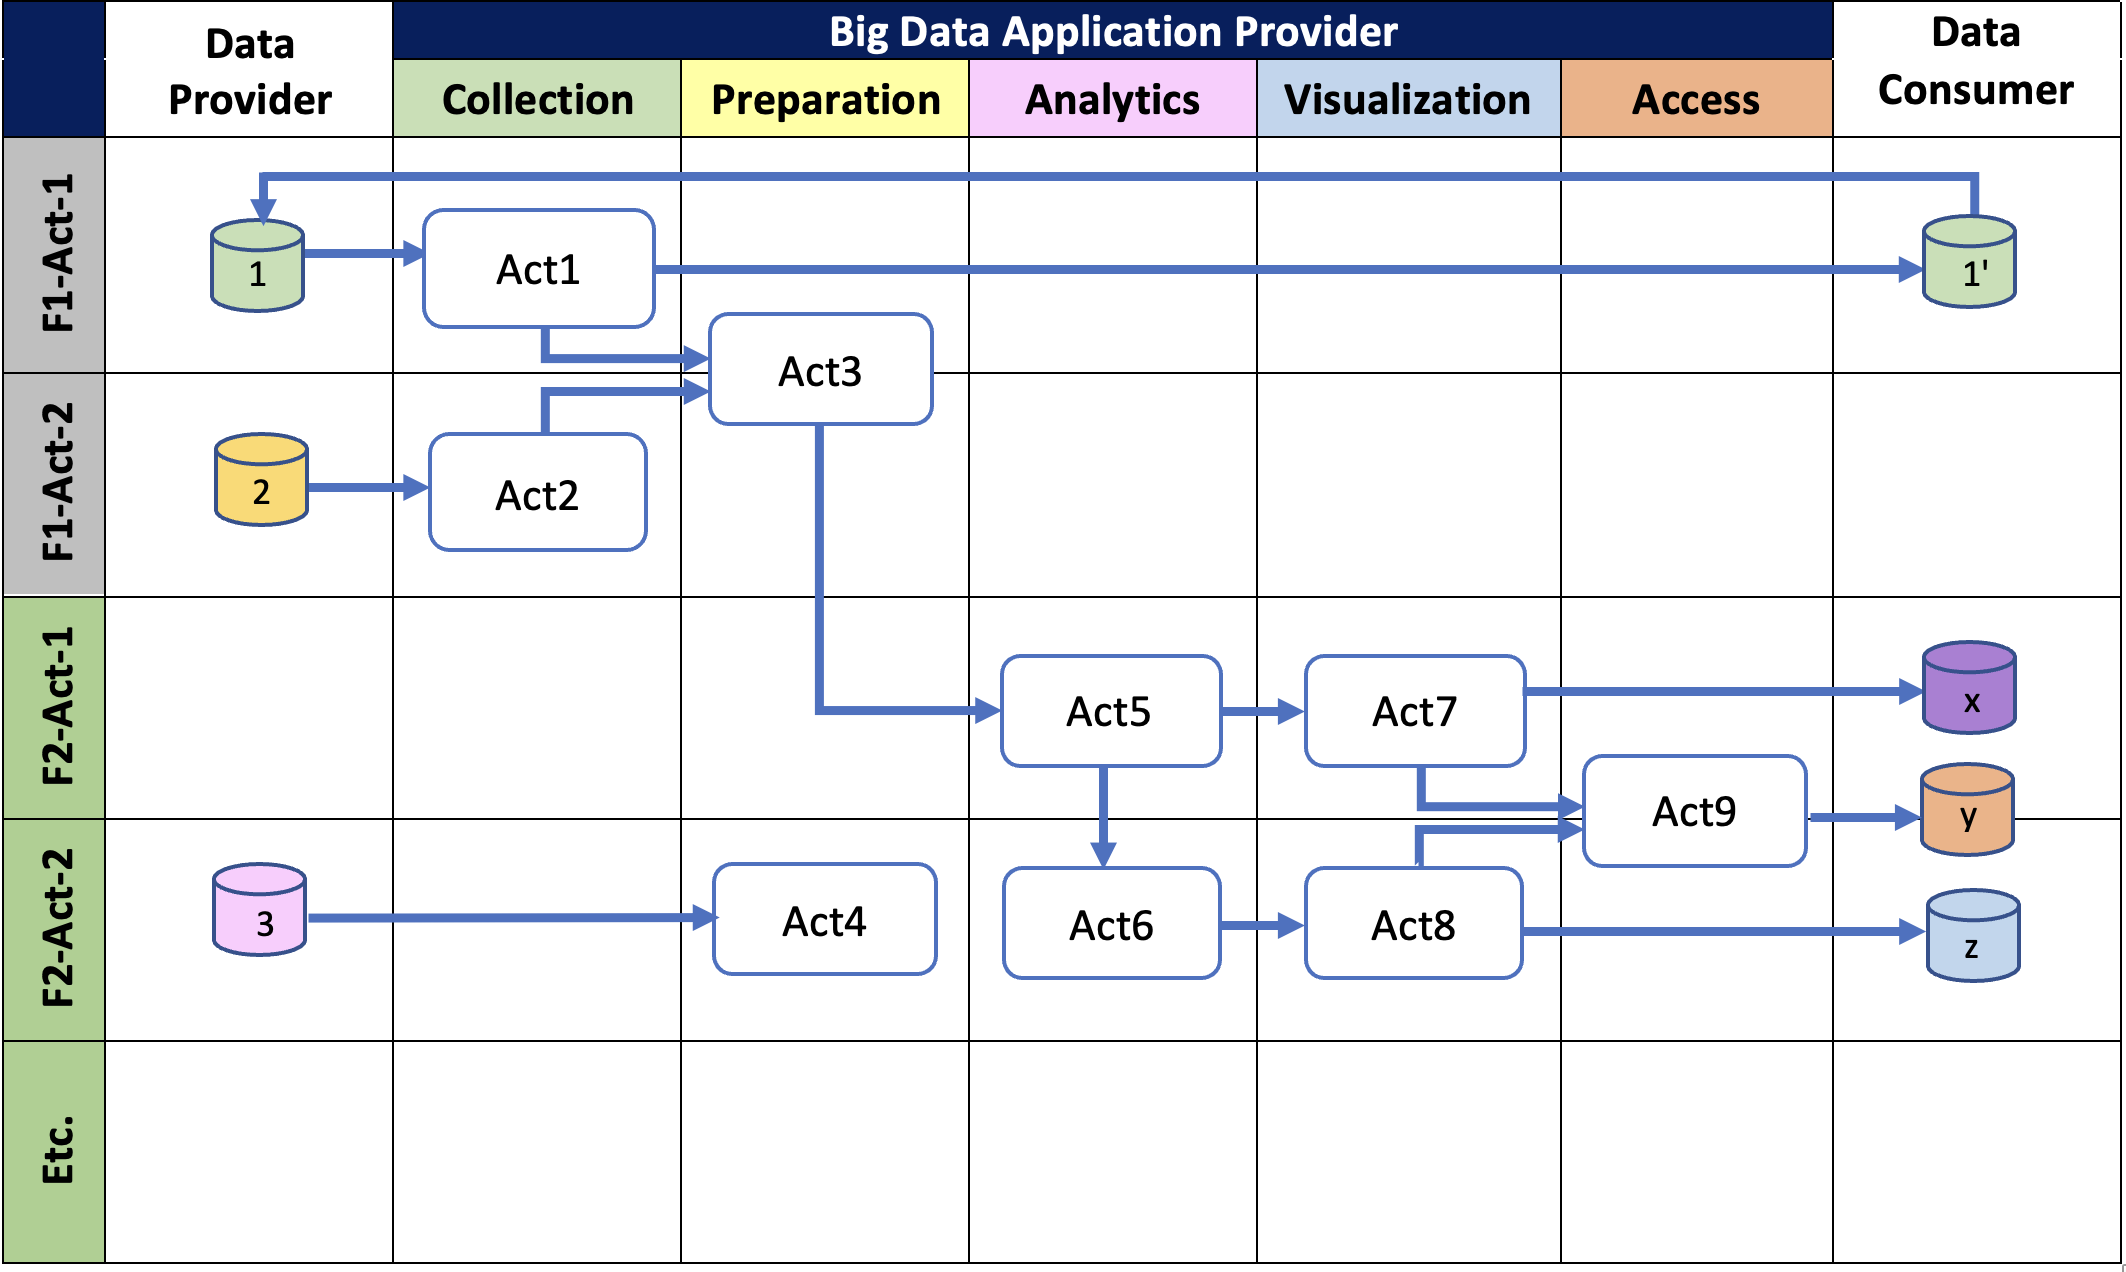
\includegraphics[width=1.0\columnwidth]{images/cross-functional-diagram.png}
    \caption{Cross-functional Diagram}
    \label{fig:cross-functional-diagram}
\end{figure}


Next, we will list use case summaries and if available point to specific publications on the NBDIF Web page that include more details. The expectation of this section is to
 
\begin{itemize}
\item	Provide an overview of use cases that motivate this document
\item	It will summarize requirements that we obtain from these use cases that influence how we proceed.
\end{itemize}

As a result, we identify how they fit into the workflow of data analytics. This includes the description of a subset of functionality that is used in general by data analytics.  In particular, it described the relationship between input and output of data analytics components and interfaces.  The use case summaries are expected to be available through the BigDataWG Web page and includes currently the following examples:

\begin{enumerate}
\item	\href{https://bigdatawg.nist.gov/_uploadfiles/M0701_v1_2020102001.docx}{M0701} -- Use case template \cite{nist-usecase-template}
\item	\href{https://bigdatawg.nist.gov/_uploadfiles/M0702_v1_2020102002.pdf}{M0702} -- Numeric weather prediction \cite{nist-wrf}
\item	\href{https://bigdatawg.nist.gov/_uploadfiles/M0703_v1_2020102003.pdf}{M0703} -- HVAC Heat ventilation and air conditioning \cite{nist-hvac}
\end{enumerate}



\FILE{usecase/weather.tex}
\subsection{Use Case: Numeric Weather Prediction}

\paragraph*{Background.} Large amounts of weather data ar e produced continually and stored in
many different databases.  Accurate weather predictions require large
amount s of processing power to accurately simulate conditions
worldwide at a high resolution and fre quent intervals. One of the
most computationally consuming parts of a reliable weather model is th
e microphysics scheme. The current microphysics scheme, Weather
Research and Forecasting (WRF) Single Moment 6-class Microphysics
(WSM6), simulates the processes in the atmosphere that leadto the
formation and precipitation of rain, snow, and graupel and requires
complex floating-point operations needing to be performed on vast
amounts of data for accurate simulations. As computer
performanceimproves, so does the Numerical Weather Prediction (NWP)
models' resolution and accuracy. However, there is still much progress
to be made, as simulation accuracy still falls off sign ificantly for
predictions more than 36 hours in advance. Figure \ref{fig:weather-1}
shows the general WRF modeling system flow chat.

\begin{figure}[htb]
\centering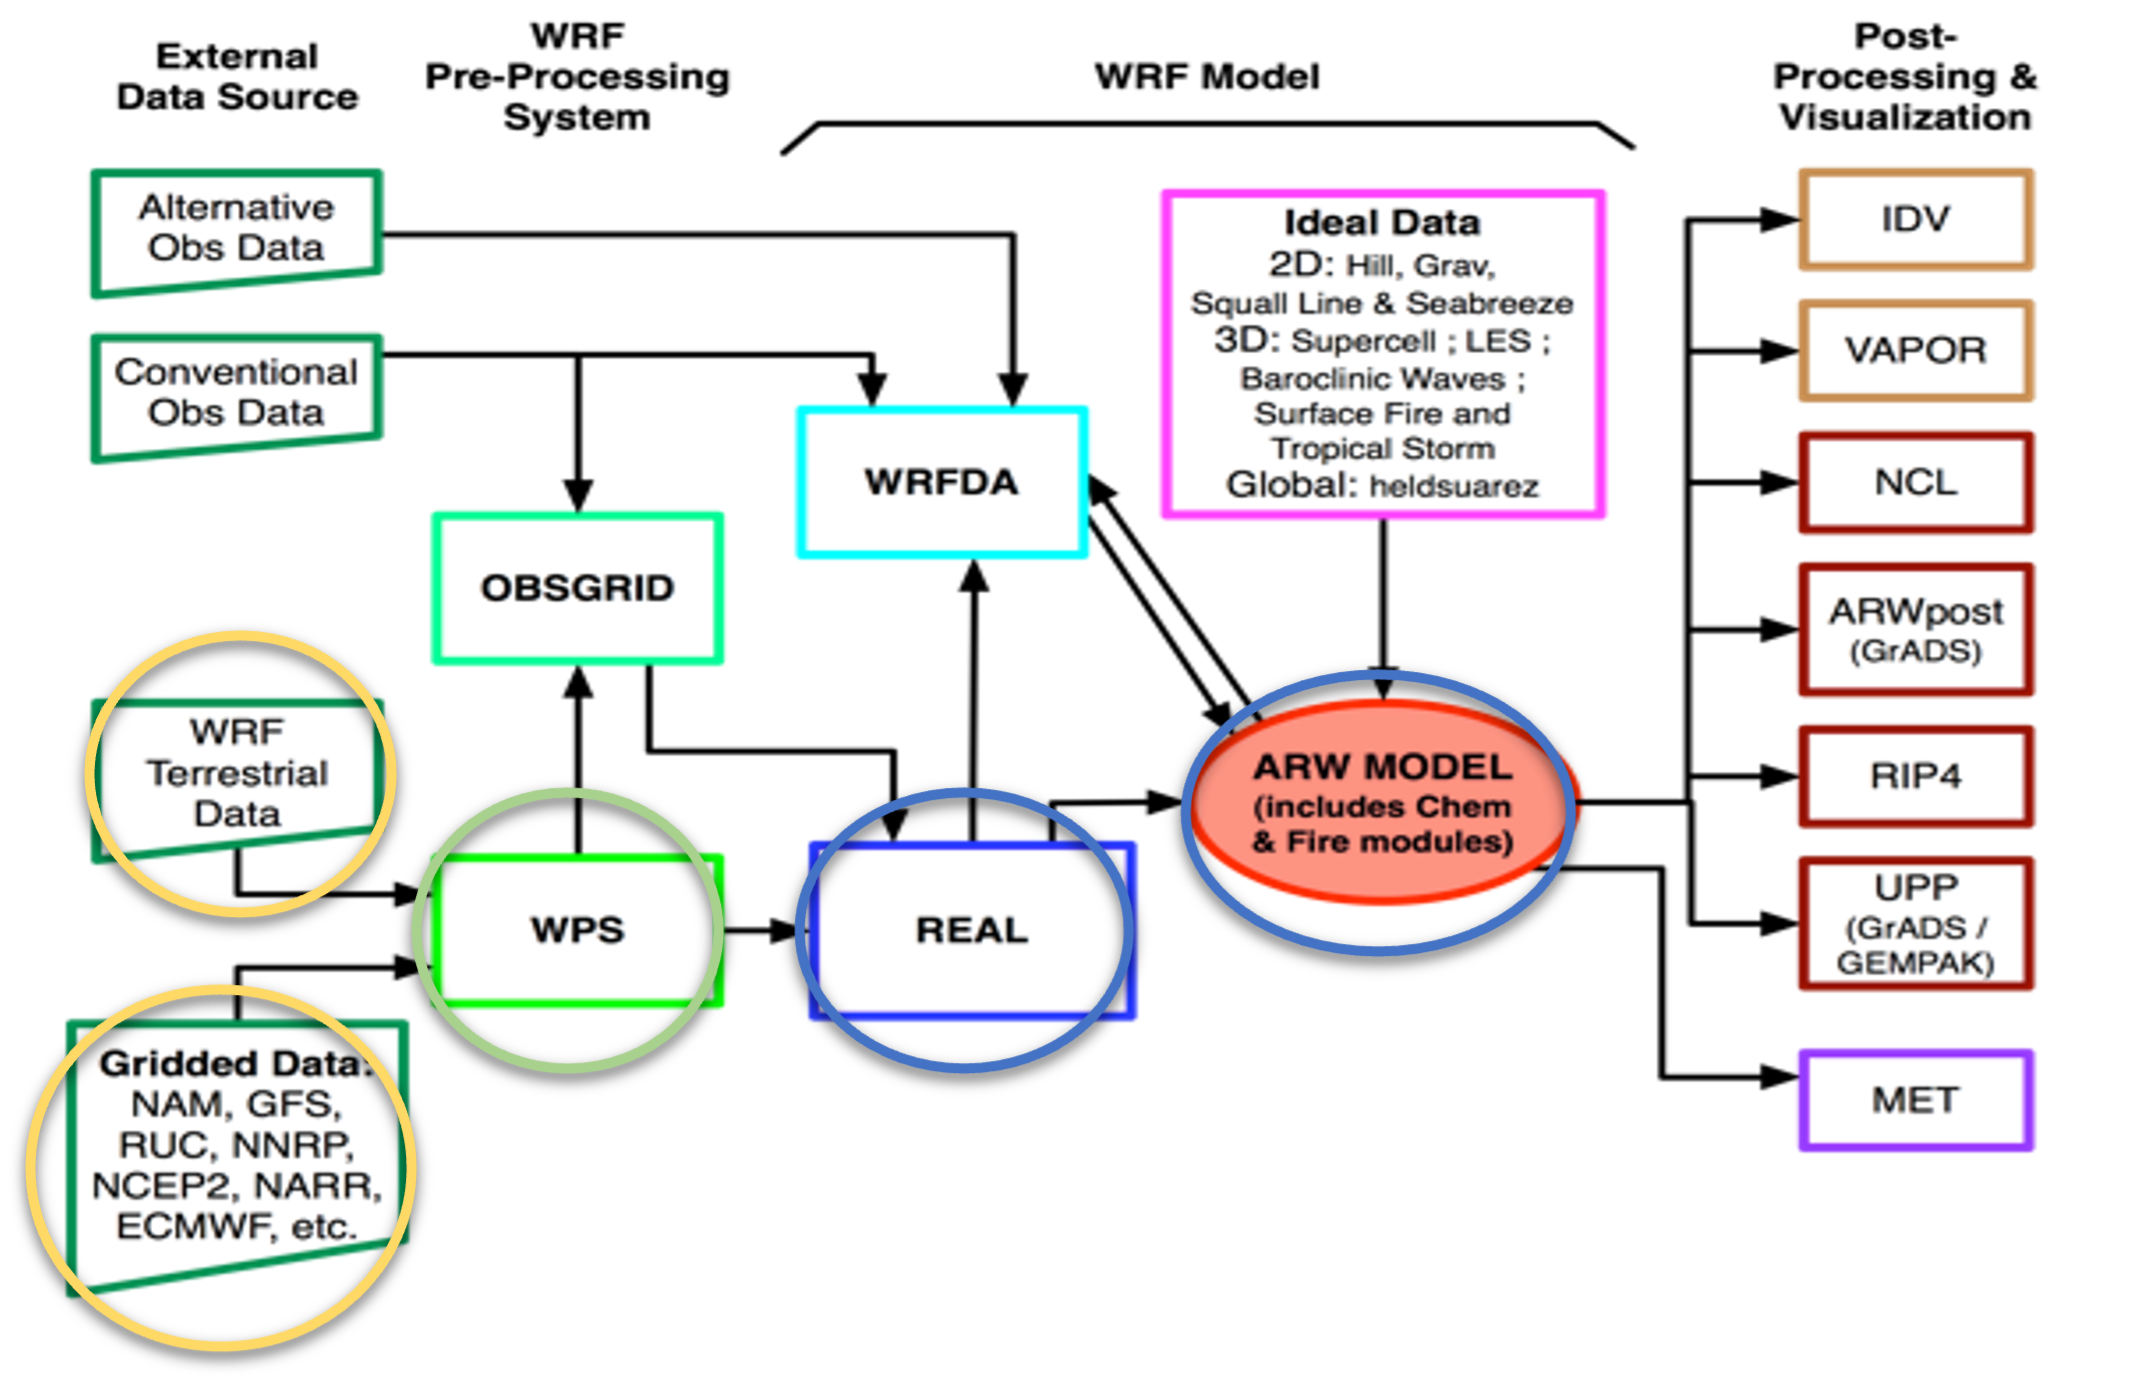
\includegraphics[width=1.0\columnwidth]{usecase/nwp-arch.png}
\label{fig:weather-1}
\caption{WRF Modeling System Flow Chart with Various Configuration.} 
\end{figure}

\paragraph*{Functionalities and Activities} (based on Big Data Application Provider of NBDIF Ref. Architecture).
In this case study, we only focus on two main functionalities, namely
WPS and WRF, and their activities.  Figure \ref{fig:weather-2} shows
the cross-functional diagram for their actions.

WPS Activities:

\begin{figure}[htb]
\centering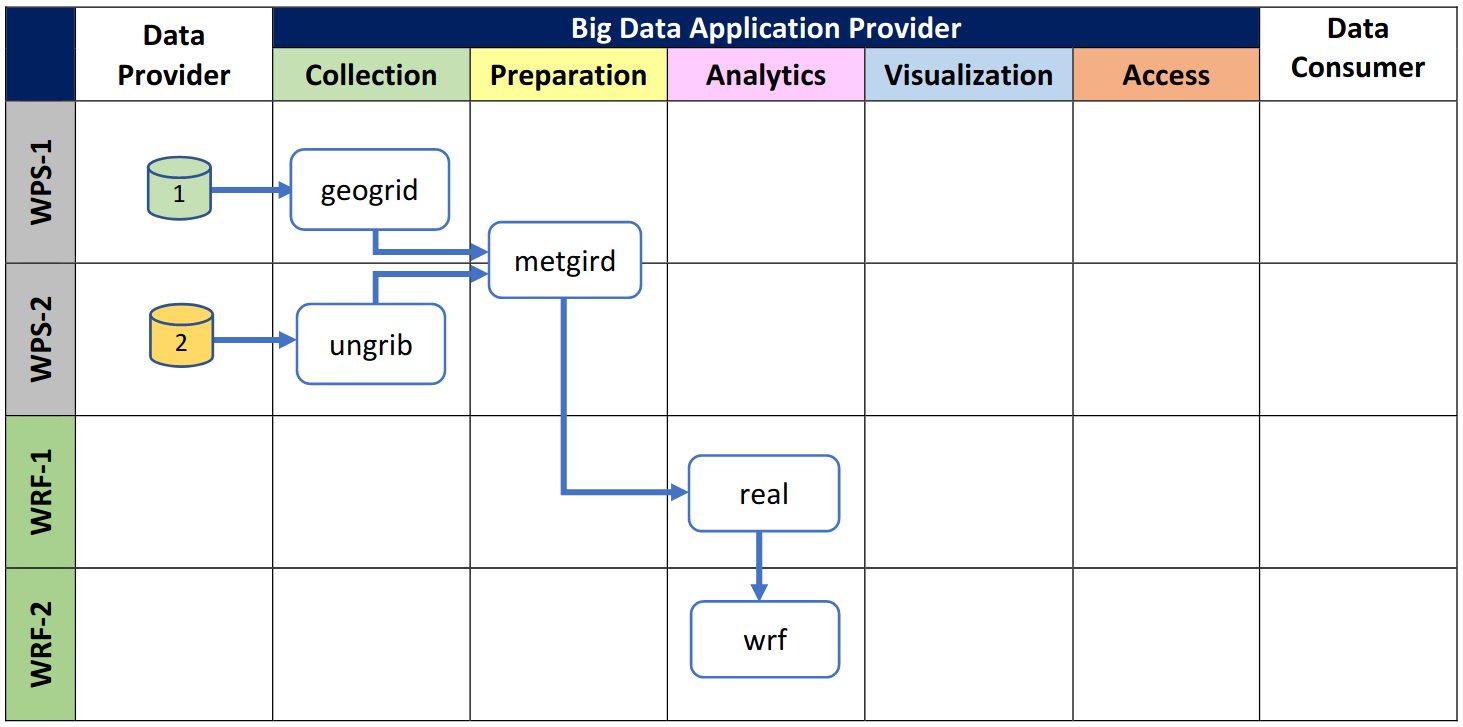
\includegraphics[width=1.0\columnwidth]{usecase/weather.png}
\label{fig:weather-2}
\caption{Cross-Functional Diagram Numerical Weather Prediction.}
\end{figure}

\begin{enumerate}
  
\item geogrid -- defines simulation domains and interpolate various terrestrial data sets to the
model grids. Input data available at [1].

\item ungrib -- extracts needed meteorological data and packs it into an intermediate file format.
Input data available at [2]

\item medgrid -- prepares horizontally interpolate the meteorological data onto the model domain.
  Input data from the output of geogrid and ungrib.

\end{enumerate}

WRF Activities:

\begin{enumerate}

\item real -- prepares vertically interpolates the output from metgrid, and creates a boundary and initial
condition files with some consistency checks.

\item wrf -- generates a model forecast.

\end{enumerate}

\paragraph*{Datasets.}

\begin{enumerate}
  
\item WRF Users Page, WPS V4 Geographical Static Data Downloads Page \cite{wrf-data}

\item NCEP FNL Operational Model Global Tropospheric Analyses, continuing
from July 1999 \cite{cisl_rda_ds083.2}

\end{enumerate}

\FILE{usecase/hvac.tex}
\subsection{Use Case: HVAC Recommendation}

\TODO{??}{move to authors: Olivera Kotevska, Research Scientist, Oak Ridge National Laboratory, U.S.A.}

\paragraph*{Background.}

Continuous streaming data is produced by heat ventilation and air conditioning (HVAC) systems every
day from the residential houses. This data is stored in a databased on the cloud as it arrives. The data
is used to calculate what should be the next HVAC set point in the house with respect to user
preferences. Periodic recommendations considering environmental parameters, user comfort level
and past user preferences require advanced machine learning algorithm called reinforcement
learning [this sentence needs grammar edit]. Accurate recommendations can save energy and reduce cost. This functionality has three
parts Environmental Forecasting (EF), Learning from the past, (LP), and Set-Point Recommendation
(SPR). EF calculates weather temperature and price predictions. LP learns from the behavior in the
past. SPR model calculates next set-point based on past experience and EF predictions. Figure \ref{fig:hvac-1} shows
the general modeling system flow chat.

\begin{figure}[htb]
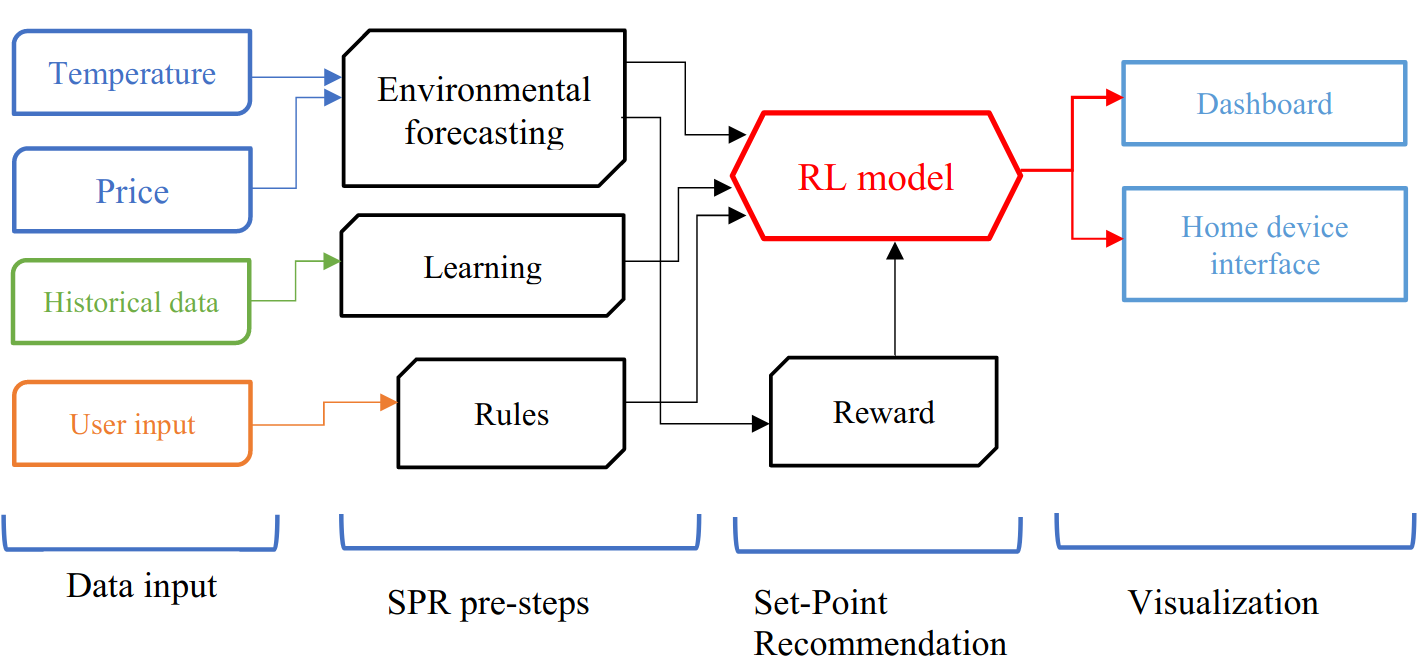
\includegraphics[width=1.0\textwidth]{usecase/hvac.png}
\label{fig:hvac-1}
\caption{HVAC general modeling system flow chat.}
\end{figure}


\paragraph*{Functionalities and Activities} (based on Big Data Application Provider of NBDIF Ref. Architecture).


In this case study, we only focus on three main functionalities, namely EF, LP and SPR, and their
activities. Figure \ref{fig:hvac-2} shows the cross-functional diagram for their actions.



\begin{figure}[htb]
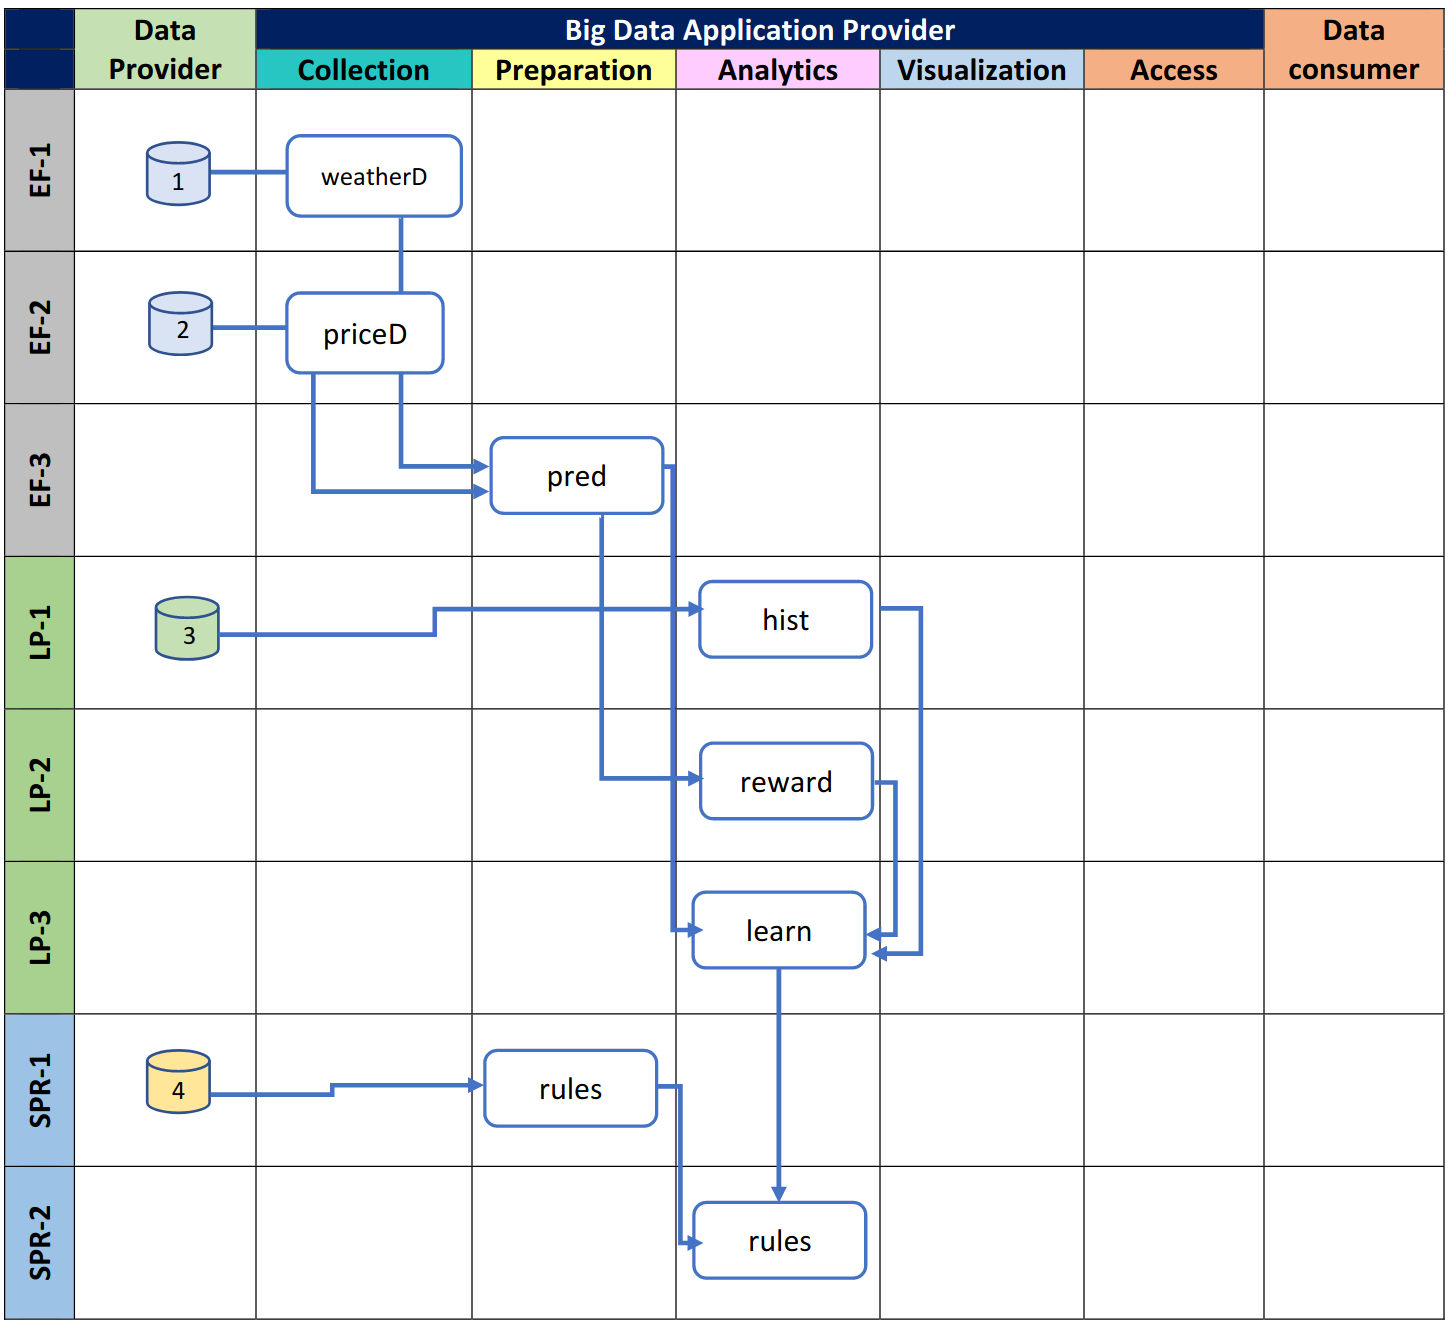
\includegraphics[width=1.0\textwidth]{usecase/hvac-2.png}
\label{fig:hvac-2}
\caption{Cross-Functional Diagram HVAC Recommendation.}
\end{figure}


EF Activities:

\begin{enumerate}
\item weatherD – Collects current weather temperature and predicted temperature for timestamp
X.
\item priceD – Collects current electricity price and predicted price for timestamp X.
\item pred – Extract needed data fields and packs it into an intermediate file format. Input data
from the output of weatherD and priceD.
\end{enumerate}


LP Activities:

\begin{enumerate}
\item hist – Prepares history data points and creates initial condition weights.
\item reward – Generates reward based on the current weatherD and priceD.
\item learn – Collects data from current weatherD, priced, reward.
\end{enumerate}

SPR Activities:

\begin{enumerate}
\item rules – Creates rules based on user preferences and conversion preferences.
\item rlmodel – Interpolates the output from learn, rules and generates set point recommendation
\end{enumerate}

\TODO{??}{No datasets provided.}

